\documentclass{beamer}

% Font selection
\usepackage{palatino}

% Beamer template
\usetheme{Antibes}
%\usetheme{Berlin}

\usepackage[scale=1.2]{ccicons}

\usepackage[utf8]{inputenc}
\usepackage[T1]{fontenc}

\usepackage{tabularx}
\usepackage{multicol}
\usepackage{graphicx}
\usepackage[final]{pdfpages}

\usepackage{listings}

\lstset{
  language=C++,
  columns=flexible,
  identifierstyle=\itshape,
%
  belowcaptionskip=1\baselineskip,
  breaklines=true,
  xleftmargin=\parindent,
  language=C++,
  showstringspaces=false,
  basicstyle=\tiny,
  keywordstyle=\bfseries\color{green!40!black},
  commentstyle=\itshape\color{purple!40!black},
  identifierstyle=\color{blue},
  stringstyle=\color{brown},
  columns=flexible,
%  inputenconding=utf8,
  extendedchars=true,
%
  morekeywords=[1]{constexpr,nullptr,alignof,alignas,decltype},
  literate={%
    {¿}{{?`}}1
    {¡}{{!`}}1
    {á}{{\'a}}1
    {é}{{\'e}}1
    {í}{{\'i}}1
    {ó}{{\'o}}1
    {ú}{{\'u}}1
    {ñ}{{\~n}}1
}
}

\newcommand{\cppkey}[1]{%
{\color{green!40!black}\texttt{#1}}%
}

\newcommand{\cppid}[1]{%
{\color{blue}\texttt{#1}}%
}

\lstdefinestyle{terminal}{
  language=bash,
  basicstyle=\scriptsize\ttfamily,
  numbersep=3pt,
  frame=tb,
  columns=fullflexible,
  backgroundcolor=\color{yellow!20},
  literate=%
    {¿}{{?`}}1
    {¡}{{!`}}1
    {á}{{\'a}}1
    {é}{{\'e}}1
    {í}{{\'i}}1
    {ó}{{\'o}}1
    {ú}{{\'u}}1
    {ñ}{{\~n}}1
}


\usepackage{listings}

\lstdefinestyle{terminal}{
  language=bash,
  basicstyle=\scriptsize\ttfamily,
  numbersep=3pt,
  frame=tb,
  columns=fullflexible,
  backgroundcolor=\color{yellow!20},
  literate=%
    {¿}{{?`}}1
    {¡}{{!`}}1
    {á}{{\'a}}1
    {é}{{\'e}}1
    {í}{{\'i}}1
    {ó}{{\'o}}1
    {ú}{{\'u}}1
    {ñ}{{\~n}}1
}

\lstdefinestyle{termoutput}{
  basicstyle=\scriptsize\ttfamily,
  frame=tb,
  backgroundcolor=\color{blue!20},
  keywordstyle=\color{black},
  commentstyle=\color{black},
  identifierstyle=\color{black},
  stringstyle=\color{black},
}


\lstset{
  language=[ISO]C++,
  basicstyle=\scriptsize,
  morekeywords=[1]{constexpr,nullptr,alignof,alignas,decltype,noexcept,override,final},
}


\renewcommand{\cppkey}[1]{%
{\color{green!40!black}\textbf{#1}}%
}

\renewcommand{\cppid}[1]{%
{\color{blue}\textbf{#1}}%
}


\usepackage{tikz}
\usetikzlibrary{positioning}
\usetikzlibrary{arrows}
\usetikzlibrary{mindmap}

\usepackage{pgfplots}
\pgfplotsset{compat=1.5}


\newcommand{\textgood}[1]{%
{\color{blue}\textbf{#1}}%
}

\newcommand{\textbad}[1]{%
{\color{red}\textbf{#1}}%
}

\newcommand{\textenum}[1]{%
{\color{blue!60!black}\textbf{#1}}%
}

\newcommand{\textmark}[1]{%
{\color{orange!70!black}\textbf{#1}}%
}




% Footline in every slide
\setbeamertemplate{footline}{
  \leavevmode%
  \hbox{\begin{beamercolorbox}[wd=\paperwidth,ht=2.5ex,dp=1.125ex,leftskip=.3cm,rightskip=.3cm]{author in head/foot}%
    \usebeamerfont{author in head/foot}\ccbyncndeu 
     \quad -- \quad J. Daniel Garcia 
     -- ARCOS@UC3M (\textbf{\url{josedaniel.garcia@uc3m.es}}) 
     -- Twitter: \textbf{\url{@jdgarciauc3m}}
    \hfill
    \insertframenumber/\inserttotalframenumber
  \end{beamercolorbox}}%
  \vskip0pt%
}

% Logo in every slide
\addtobeamertemplate{headline}{}
{% 
\begin{tikzpicture}[remember picture,overlay]
\node[anchor=north east] at (current page.north east) {\includegraphics[height=0.7cm]{logos/arcos_t.png}};
\end{tikzpicture}
}

\tikzset{
  invisible/.style={opacity=0},
  visible on/.style={alt=#1{}{invisible}},
  alt/.code args={<#1>#2#3}{%
    \alt<#1>{\pgfkeysalso{#2}}{\pgfkeysalso{#3}} % \pgfkeysalso doesn't change the path
  },
}

%Portada
\title{GrPPI}
\subtitle{Generic Reusable Parallel Patterns Interface}
\author{J. Daniel Garcia}
\institute{ARCOS Group\\University Carlos III of Madrid\\Spain}
\date{October 2017}

\begin{document}

\begin{frame}
\titlepage
\end{frame}

\AtBeginSection[]
{
  \begin{frame}<*>
    \setbeamertemplate{section in toc shaded}[default][50]
    \setbeamertemplate{subsection in toc shaded}[default][50]
    \tableofcontents[currentsection,hideallsubsections]
  \end{frame}
}

\AtBeginSubsection[]
{
  \begin{frame}<beamer>
    \setbeamertemplate{subsection in toc shaded}[default][50]
    \tableofcontents[sectionstyle=show/hide,subsectionstyle=show/shaded/hide]
  \end{frame}
}

\begin{frame}{Warning}

\begin{tabularx}{.98\textwidth}{lX}
\ccLogo & This work is under 
Attribution-NonCommercial-NoDerivatives 4.0 International (CC BY-NC-ND 4.0) license.\\

& You are \textbf{free} to
\textbf{Share} — copy and redistribute the material in any medium or format.
\\

\ccAttribution & 
You must give appropriate credit, provide a link to the license, and indicate if changes were made. You may do so in any reasonable manner, but not in any way that suggests the licensor endorses you or your use.\\

\ccNonCommercialEU &
You may not use the material for commercial purposes.
\\

\ccNoDerivatives &
If you remix, transform, or build upon the material, you may not distribute the modified material.
\\

\end{tabularx}

\end{frame}

\begin{frame}{ARCOS@uc3m}
\begin{itemize}
  \item \textbf{UC3M}: A young international research oriented university.
  \vfill
  \item \textbf{ARCOS}: An applied research group.
    \begin{itemize}
      \item {\color{blue}{Lines}}: 
        High Performance Computing,
        Big data,
        Cyberphysical Systems, and
        \textmark{Programming models for application improvement}.
    \end{itemize} 
  \vfill
  \item \textbf{Improving applications}:
    \begin{itemize}
      \item \textmark{REPARA}: Reengineering and Enabling Performance and poweR of Applications.
            Financiado por Comisión Europea (FP7). 2013--2016
      \item \textmark{RePhrase}: REfactoring Parallel Heterogeneous Resource Aware Applications.
            Financiado por Comisión Europea (H2020). 2015--2018
    \end{itemize} 
  \vfill
  \item \textbf{Standardization}:
    \begin{itemize}
      \item \textgood{ISO/IEC JTC/SC22/WG21}. ISO C++ standards committe.
    \end{itemize}
\end{itemize}
\end{frame}

\begin{frame}[t]{Acknowledgements}
\begin{itemize}
  \item The GrPPI library has been partially supported by:
    \begin{itemize}
      \vfill
      \item Project ICT 644235 \textmark{``REPHRASE: REfactoring Parallel Heterogeneous Resource-aware Applications''} 
            funded by the European Commission through H2020 program (2015-2018).
      \vfill
      \item Project TIN2016-79673-P \textmark{``Towards Unification of HPC and Big Data Paradigms''} 
            funded by the Spanish Ministry of Economy and Competitiveness (2016-2019).
    \end{itemize}
\end{itemize}

\vfill
\begin{center}
\includegraphics[height=1cm]{logos/rephrase.jpg}
\hspace{1cm}
\includegraphics[height=1.5cm]{logos/bighpc.png}
\end{center}
\end{frame}


\section{Introduction}

\begin{frame}[t]{Sequential Programming versus Parallel Programming}
\begin{itemize}
\item \textmark{Sequential programming}
  \begin{itemize}
    \item Well-known set of \emph{control-structures} embedded in programming languages.
    \item Control structures inherently sequential.
  \end{itemize}
\vfill\pause
\item \textmark{Traditional Parallel programming}
  \begin{itemize}
    \item Constructs \emph{adapting} sequential control structures to the parallel world
          (e.g. \emph{parallel-for}).
  \end{itemize}
\vfill\pause
\item But wait!
  \begin{itemize}
    \item What if we had constructs that could be both sequential and parallel?
  \end{itemize}
\end{itemize}
\end{frame}

\begin{frame}[t]{Software design}

\begin{quote}
There are two ways of constructing a software design:\\ 
\vspace{1em}
\pause
One way is\\
\pause
to make it \textgood{so simple} that there are \textmark{obviously no deficiencies},\\
\pause
\vspace{.5em}
and the other way is\\
\pause
to make it \textgood{so complicated} that there are \textmark{no obvious deficiencies}.\\ 
\vspace{1em}
\pause
The \textmark{first method} is \textbad{far more difficult}. 
\end{quote}
\hfill C.A.R Hoare
\end{frame}

\begin{frame}[t,fragile]{Adding two vectors}
\begin{block}{Traditional way}
\lstinputlisting[firstline=6,lastline=15]{ej/src/addvec/classic.cpp}
\end{block}
\pause
\begin{itemize}
  \item Adds additional constraints.
    \begin{itemize}
      \item Traversing in-order.
    \end{itemize}
  \item Potential mistakes.
    \begin{itemize}
      \item \cppid{i<v1.size()} versus \cppid{i<=v1.size()}.
    \end{itemize}
\end{itemize}
\end{frame}

\begin{frame}[t,fragile]{Adding two vectors}
\begin{block}{The STL way (C++98/03)}
\lstinputlisting[firstline=6,lastline=15]{ej/src/addvec/stl.cpp}
\end{block}
\pause
\begin{itemize}
  \item Minimize off-by-one mistakes.
  \item Type specific optimizations.
\end{itemize}
\end{frame}

\begin{frame}[t,fragile]{Adding two vectors}
\begin{block}{The STL way (C++14)}
\lstinputlisting[firstline=6,lastline=15]{ej/src/addvec/stl11.cpp}
\end{block}
\pause
\begin{itemize}
  \item Use (possibly generic) lambdas .
\end{itemize}
\end{frame}

\begin{frame}[t]{A brief history of patterns}
\begin{itemize}
\item From building and architecture (Cristopher Alexander):
\begin{itemize}
  \item \textbf{1977}: A Pattern Language: Towns, Buildings, Construction.
  \item \textbf{1979}: The timeless way of buildings.
\end{itemize}
\pause\vfill
\item To software design (Gamma et al.):
\begin{itemize}
  \item \textbf{1993}: Design Patterns: abstraction and reuse of object oriented design. ECOOP.
  \item \textbf{1995}: Design Patterns. Elements of Reusable Object-Oriented Software.
\end{itemize}
\pause\vfill
\item To parallel programming (McCool, Reinders, Robinson):
\begin{itemize}
  \item \textbf{2012}: Structured Parallel Programming: Patterns for Efficient Computation.
\end{itemize}
\end{itemize}
\end{frame}

\begin{frame}[t]{Parallel Patterns}
\begin{itemize}
  \item Levels of patterns:
    \begin{itemize}
      \item Software Architecture Patterns.
      \item Design Patterns.
      \item Algorithm Strategy Patterns.
      \item Implementation patterns.
    \end{itemize}

  \vfill\pause
  \item \textmark{Algorithm Strategy Pattern} or \textmark{Algorithmic Skeleton}
    \begin{itemize}
      \item A way to codify best practices in \textmark{parallel programming} 
            in a \textgood{reusable way}.
    \end{itemize}

  \vfill\pause
  \item A single \textmark{Parallel Pattern} may have \textgood{different realizations}
        in \textgood{different programming models}.
  
\end{itemize}
\end{frame}

\begin{frame}[t,fragile]{Example: map pattern}
\begin{itemize}
  \item Apply a single \textmark{elemental operation} to different \textmark{data items}.
\end{itemize}
\begin{columns}

\column{.5\textwidth}
\begin{block}{SAXPY: Sequential}
\begin{lstlisting}
for (size_t i=0; i<n; ++i) {
  y[i] = a * x[i] + y[i];
}
\end{lstlisting}
\end{block}

\pause

\begin{block}{SAXPY: OpenMP}
\begin{lstlisting}
#pragma omp parallel for
for (size_t i=0; i<n; ++i) {
  y[i] = a * x[i] + y[i];
}
\end{lstlisting}
\end{block}

\pause

\column{.5\textwidth}
\begin{block}{SAXPY: Sequential}
\begin{lstlisting}
tbb::parallel_for(tbb::blocked_range<int>{0,n},
  [&](tbb::blocked_range<int> r) {
    for (auto i : r) {
      y[i] = a * x[i] + y[i];
    }
  });
\end{lstlisting}
\end{block}
\end{columns}
\end{frame}

\subsection{GrPPI architecture}

\begin{frame}[t]{Some ideals}
\begin{itemize}[<+->]
  \item Applications should be expressed independently of the
        execution model.
  \item Multiple back-ends should be offered with simple switching
        mechanisms.
  \item Interface should integrate seamlessly with modern C++ standard
        library.
  \item Make use of modern (C++14) language features.
\end{itemize}
\end{frame}

\begin{frame}[t]{GrPPI}
\begin{Large}
\textgood{\url{https://github.com/arcosuc3m/grppi}}
\end{Large}
\vfill\pause
\begin{itemize}
  \item A header only library (might change).
  \item A set of execution policies.
  \item A set of type safe generic algorithms.
  \item Requires \textgood{C++14}.
  \item GNU GPL v3.
\end{itemize}
\end{frame}

\begin{frame}[t,fragile]{Setting up GrPPI}
\begin{itemize}
  \item \textenum{Structure}.
    \begin{itemize}
      \item \textmark{include}: Include files.
      \item \textmark{unit\_tests}: Unit tests using GoogleTest.
      \item \textmark{samples}: Sample programs.
      \item \textmark{cmake-modules}: Extra CMake scripts.
    \end{itemize}
  \vfill\pause
  \item Initial setup
\begin{lstlisting}[style=terminal]
mkdir build
cd build
cmake ..
make
\end{lstlisting}
\end{itemize}
\end{frame}

\begin{frame}[t]{CMake variables}
\begin{itemize}
  \item \textmark{GRPPI\_UNIT\_TESTS\_ENABLE}: Enable building unit tests.
  \item \textmark{GRPPI\_OMP\_ENABLE}: Enable OpenMP back-end.
  \item \textmark{GRPPI\_TBB\_ENABLE}: Enable Intel TBB back-end.
  \item \textmark{GRPPI\_EXAMPLE\_APPLICATIONS\_ENABLE}: Enable building example applications.
  \item \textmark{GRPPI\_DOXY\_ENABLE}: Enable documentation generation.
\end{itemize}
\end{frame}

\begin{frame}[t]{Execution policies}
\begin{itemize}
  \item The execution model is encapsulated by execution values.
  \vfill
  \item Current execution types:
    \begin{itemize}
      \item \cppid{sequential\_execution}.
      \item \cppid{parallel\_execution\_native}.
      \item \cppid{parallel\_execution\_omp}.
      \item \cppid{parallel\_execution\_tbb}.
      \item \cppid{dynamic\_execution}.
    \end{itemize}
  \vfill
  \item All top-level patterns take one \emph{execution} object.
\end{itemize}
\end{frame}

\begin{frame}[t]{Concurrency degree}
\begin{itemize}
  \item Sets the number of underlying threads used by the execution implementation.
    \begin{itemize}
      \item \cppid{sequential\_execution} $\Rightarrow$ 1
      \item \cppid{parallel\_execution\_native} $\Rightarrow$ \cppid{hardware\_concurrency()}.
      \item \cppid{parallel\_execution\_omp} $\Rightarrow$ \cppid{omp\_get\_num\_threads()}.
    \end{itemize}

  \vfill
  \item \textenum{API}
    \begin{itemize}
      \item \cppid{ex.set\_concurrency\_degree(4)}
      \item \cppkey{int }\cppid{n = ex.concurrency\_degree()}
    \end{itemize}
\end{itemize}
\end{frame}

\begin{frame}[t,fragile]{Dynamic back-end}
\begin{itemize}
  \item Useful if you want to take the decision at run-time.
  \item Holds any other execution policy (or empty).
\end{itemize}
\vfill\pause
\begin{block}{Selecting the execution back-end}
\begin{lstlisting}
grppi::dynamic_execution execution_mode(const std::string & opt) {
  using namespace grppi;
  if ("seq" == opt) return sequential_execution{};
  if ("thr" == opt) return parallel_execution_native{};
  if ("omp" == opt) return parallel_execution_omp{};
  if ("tbb" == opt) return parallel_execution_tbb{};
  return {};
}
\end{lstlisting}
\end{block}
\end{frame}

\begin{frame}[t]{Function objects}
\begin{itemize}
  \item GrPPI is heavily based on passing code sections as function objects
        (aka \emph{functors}).
  \vfill
  \item \textenum{Alternatives}:
    \begin{itemize}
      \item Standard C++ predefined functors (e.g. \cppid{std::plus<int>}).
      \item Custom hand-written function objects.
      \item Lambda expressions.
    \end{itemize}
  \vfill
  \item Usually lambda expressions lead to more concise code.
\end{itemize}
\end{frame}



\subsection{Data patterns}

\begin{frame}[t]{Patterns on data sets}
\begin{itemize}
  \item A \textgood{data pattern} performs an operation on one 
        or more data sets that are already in memory.

  \vfill 
  \item \textmark{Input}:
    \begin{itemize}
      \item One or more data sets.
      \item Operations.
    \end{itemize}

  \vfill 
  \item \textmark{Output}:
    \begin{itemize}
      \item A data set (\cppid{map}, \cppid{stencil}).
      \item A single value (\cppid{reduce}, \cppid{map/reduce}).
    \end{itemize}
\end{itemize}
\end{frame}

\begin{frame}[t]{Maps on data sequences}
\begin{itemize}
  \item A \textgood{map} pattern applies an operation to every element in a
        a data set, generating a new data set.
  \vfill
  \item \textgood{Unidimensional}:
    \begin{itemize}
      \item $S = x_1, x_2, \ldots x_n$
      \item $map(S,f)$
        \begin{itemize} 
          \item $f(x_1), f(x_2), \ldots, f(x_n)$
        \end{itemize}
    \end{itemize}

  \vfill
  \item \textgood{Multidimensional}:
    \begin{itemize}
      \item $S_k = x^k_1, x^k_2, \ldots, x^k_n$
      \item $map(S_1, S_2, \ldots, S_m, f)$
        \begin{itemize}
          \item $f(x^1_1, x^2_1, \ldots, x^m_1), f(x^2_1, x^2_2, \ldots, x^m_2), \ldots$
        \end{itemize}
    \end{itemize}
\end{itemize}
\end{frame}

\begin{frame}[t,fragile]{Single sequences mapping}
\begin{block}{Double all elements in sequence}
\begin{lstlisting}
template <typename Execution>
std::vector<double> double_elements(const Execution & ex, 
                                    const std::vector<double> & v) 
{
  std::vector<double> res(v.size());

  grppi::map(ex, v.begin(), v.end(), res.begin(), 
    [](double x) { return 2*x; });

  return res;
}
\end{lstlisting}
\end{block}
\end{frame}

\begin{frame}[t,fragile]{Multiple sequences mapping}
\begin{block}{Add two vectors}
\begin{lstlisting}
template <typename Execution>
std::vector<double> add_vectors(const Execution & ex, 
                                const std::vector<double> & v1,
                                const std::vector<double> & v2) 
{
  auto size = std::min(v1.size(), v2.size());
  std::vector<double> res(size);

  grppi::map(ex, v1.begin(), v1.end(), res.begin(),
    [](double x, double y) { return x+y; },
    v2.begin());

  return res;
}
\end{lstlisting}
\end{block}
\end{frame}

\begin{frame}[t,fragile]{Multiple sequences mapping}
\begin{block}{Add three vectors}
\begin{lstlisting}
template <typename Execution>
std::vector<double> add_vectors(const Execution & ex, 
                                const std::vector<double> & v1,
                                const std::vector<double> & v2,
                                const std::vector<double> & v3) 
{
  auto size = std::min(v1.size(), v2.size());
  std::vector<double> res(size);

  grppi::map(ex, v1.begin(), v1.end(), res.begin(),
    [](double x, double y, double z) { return x+y+z; },
    v2.begin(), v3.begin());

  return res;
}
\end{lstlisting}
\end{block}
\end{frame}

\begin{frame}[t,fragile]{Heterogeneous mapping}
\begin{itemize}
  \item The result can be from a different type.
\end{itemize}
\begin{block}{Complex vector from real and imaginary vectors}
\begin{lstlisting}
template <typename Execution>
std::vector<complex<double>> create_cplx(const Execution & ex,
                                         const std::vector<double> & re,
                                         const std::vector<double> & im)
{
  auto size = std::min(re.size(), im.size());
  std::vector<complex<double>> res(size);

  grppi::map(ex, re.begin(), re.end(), res.begin(),
    [](double r, double i) -> complex<double> { return {r,i}; }
    im.begin());

  return res;
}
\end{lstlisting}
\end{block}
\end{frame}

\begin{frame}[t]{Reductions on data sequences}
\begin{itemize}
  \item A \textgood{reduce} pattern combines all values in a data set
        using a binary combination operation.
  \vfill

\begin{tikzpicture}
\tikzset{
  label/.style={text centered, text=orange,font=\footnotesize,minimum width=1cm} ,
  transform/.style={rectangle,rounded corners,draw=black,fill=green!50,text=white,thick, text centered, font=\tiny, minimum width=0.75cm,minimum height=0.5cm},
  item/.style={rectangle,draw=black,fill=orange!70,text=white,thick, text centered, font=\tiny, minimum width=0.75cm},
  result/.style={rectangle,draw=black,fill=blue!70,text=white,thick, text centered, font=\tiny, minimum width=0.75cm},
  arrow/.style={->,thick,draw=black,font=\tiny},
}
\node[item,fill=orange!20,text=black] (item0) {id};
\node[item,right=1cm of item1] (item1) {};
\node[item,right=0cm of item1] (item2) {};
\node[item,right=0cm of item2] (item3) {};
\node[item,right=0cm of item3] (item4) {};
\node[item,right=0cm of item4] (item5) {};
%
\node[transform,below=0.25cm of item1,minimum width=0.5cm] (map1) {};
\node[transform,below=0.25cm of item2,minimum width=0.5cm] (map2) {};
\node[transform,below=0.25cm of item3,minimum width=0.5cm] (map3) {};
\node[transform,below=0.25cm of item4,minimum width=0.5cm] (map4) {};
\node[transform,below=0.25cm of item5,minimum width=0.5cm] (map5) {};
%
\node[result,below=0.5cm of map5] (result) {result};
%
\path[arrow](item0) -- (map1);
\path[arrow](item1) -- (map1);
\path[arrow](map1) -- (map2);
\path[arrow](item2) -- (map2);
\path[arrow](map2) -- (map3);
\path[arrow](item3) -- (map3);
\path[arrow](map3) -- (map4);
\path[arrow](item4) -- (map4);
\path[arrow](map4) -- (map5);
\path[arrow](item5) -- (map5);
%
\path[arrow](map5) -- (result);
\end{tikzpicture}


%  \item Given:
%    \begin{itemize}
%      \item A sequence $x_1, x_2, \ldots, x_N \in T$.
%      \item An identity value $id \in I$.
%      \item A combine operation $c : I \times T \mapsto I$
%        \begin{itemize}
%          \item $c(c(x,y),z) \equiv c(x,c(y,z))$
%          \item $c(id,x) = \bar{x}$, where $\bar{x}$ is the value of $x$ in $I$.
%          \item $c(id,c(id,x)) = c(id,x)$
%          \item $c(c(c(id,x),y),c(c(id,z),t)) = c(c(c(c(id,x),y),z),t)$
%        \end{itemize}
%    \end{itemize}
%  \vfill
%  \item It generates the value:
%    \begin{itemize}
%      \item $c(\ldots c(c(id,x_1), x_2) \ldots, x_N)$
%    \end{itemize}
\end{itemize}
\end{frame}

\begin{frame}[t,fragile]{Homogeneous reduction}
\begin{block}{Add a sequence of values}
\begin{lstlisting}
template <typename Execution>
double add_sequence(const Execution & ex, const vector<double> & v)
{
  return grppi::reduce(ex, v, 0.0,
    [](double x, double y) { return x+y; });
}
\end{lstlisting}
\end{block}
\end{frame}

\begin{frame}[t,fragile]{Heterogeneous reduction}
\begin{block}{Add areas of shapes}
\begin{lstlisting}
template <typename Execution>
int add_areas(const Execution & ex, const std::vector<shape> & shapes)
{
  return grppi::reduce(ex, shapes, 0.0,
    [](double a, const auto & s) { 
        return a + s.area()(); 
    });
}
\end{lstlisting}
\end{block}
\begin{itemize}
  \item \textbad{Note}: Better expressed as a map reduce.
\end{itemize}
\end{frame}

\subsection{Map/reduce pattern}

\begin{frame}[t]{Map/reduce pattern}
\begin{itemize}
  \item A \textgood{map/reduce} pattern combines a \textmark{map} pattern and
        a \textmark{reduce} pattern into a single pattern.
    \begin{enumerate}
      \item One or more data sets are \textmark{mapped} applying a transformation operation.
      \item The results are combined by a \textmark{reduction} operation.
    \end{enumerate}
  \vfill
  \item A \textmark{map/reduce} could be also expressed by the composition of a
        \textmark{map} and a \textmark{reduce}. 
    \begin{itemize}
      \item However, \textmark{map/reduce} may potentially fuse both stages, 
            allowing for extra optimizations.
    \end{itemize}
\end{itemize}
\end{frame}

\begin{frame}[t]{Map/reduce with single data set}
\begin{itemize}
  \item A \textgood{map/reduce} on a single input sequence producing a value.
  \vfill\pause
  \item Given:
    \begin{itemize}
      \item A sequence $x_1, x_2, \ldots x_N \in T$
      \item A mapping function $m : T \mapsto R$
      \item A reduction identity value $id \in I$.
      \item A combine operation $c : I \times R \mapsto I$
    \end{itemize}
  \vfill\pause
  \item It generates a value reducing the mapping:
    \begin{itemize}
      \item $c(c(c(id,m_1),m_2), \ldots, m_M)$
      \item Where $m_k = m(x_k)$
    \end{itemize}
\end{itemize}
\end{frame}

\begin{frame}[t,fragile]{Single sequence map/reduce}
\begin{block}{Sum of squares}
\begin{lstlisting}
template <typename Execution>
double sum_squares(const Execution & ex, const std::vector<double> & v)
{
  return grppi::map_reduce(ex, v.begin(), v.end(), 0.0,
    [](double x) { return x*x; }
    [](double x, double y) { return x+y; }
  );
}
\end{lstlisting}
\end{block}
\end{frame}

\begin{frame}[t]{Map/reduce in multiple data sets}
\begin{itemize}
  \item A \textgood{map/reduce} on multiple input sequences producing a single value.
  \vfill\pause
  \item Given:
    \begin{itemize}
      \item A sequence $x^1_1, x^1_2, \ldots x^1_N \in T_1$
      \item A sequence $x^2_1, x^2_2, \ldots x^2_N \in T_2$
      \item \ldots
      \item A sequence $x^M_1, x^M_2, \ldots x^M_N \in T_M$
      \item A mapping function $m : T_1 \times T_2 \times \ldots \times T_M \mapsto R$
      \item A reduction identity value $id \in I$.
      \item A combine operation $c : I \times R \mapsto I$
    \end{itemize}
  \vfill\pause
  \item It generates a value reducing the mapping:
    \begin{itemize}
      \item $c(c(c(id,m_1),m_2), \ldots, m_M)$
      \item Where $m_k = m(x^k_1, x^k_2, \ldots, x^k_N)$
    \end{itemize}
\end{itemize}
\end{frame}

\begin{frame}[t,fragile]{Map/reduce on two data sets}
\begin{block}{Scalar product}
\begin{lstlisting}
template <typename Execution>
double scalar_product(const Execution & ex,
                      const std::vector<double> & v1,
                      const std::vector<double> & v2)
{
  return grppi::map_reduce(ex, begin(v1), end(v1), 0.0,
    [](double x, double y) { return x*y; },
    [](double x, double y) { return x+y; },
    v2.begin());
}
\end{lstlisting}
\end{block}
\end{frame}

\begin{frame}[t,fragile]{Cannonical map/reduce}
\begin{itemize}
  \item Given a sequence of words, produce a \emph{<key,value>} container where:
    \begin{itemize}
      \item The key is the word.
      \item The value is the number of occurrences of that word.
    \end{itemize}
\end{itemize}
\vfill\pause
\begin{block}{Word frequencies}
\begin{lstlisting}
template <typename Execution>
auto word_freq(const Execution & ex, const std::vector<std::string> & words)
{
  using namespace std;
  using dictionary = std::map<string,int>;
  return grppi::map_reduce(ex, words.begin(), words.end(), dictionary{},
    [](string w) -> dictionary { return {w,1}; }
    [](dictionary & lhs, const dictionary & rhs) -> dictionary {
      for (auto & entry : rhs) { lhs[entry.first] += entry.second; }
      return lhs;
    });
}
\end{lstlisting}
\end{block}
\end{frame}


\section{Task Patterns}

\begin{frame}[t]{Divide/conquer pattern}
\begin{itemize}
  \item A \textgood{divide/conquer} pattern splits a problem into two or more independent subproblems until a base case is reached.
    \begin{itemize}
      \item The base case is solved directly.
      \item The results of the subproblems are combined until the final solution of the original problem is obtained.
    \end{itemize}

  \vfill\pause
  \item \textenum{Key elements}:
    \begin{itemize}
      \item \textmark{Divider}: Divides a problem in a set of subproblems.
      \item \textmark{Solver}: Solves and individual subproblem.
      \item \textmark{Combiner}: Combines two solutions.
    \end{itemize}
\end{itemize}
\end{frame}

\begin{frame}[t,fragile]{A patterned merge/sort}
\begin{block}{Ranges on vectors}
\begin{lstlisting}
struct range {
  range(std::vector<double> & v) : first{v.begin()}, last{v.end()} {}
  auto size() const { return std::distance(first,last); }
  std::vector<double> first, last;
};

std::vector<range> divide(range r) {
  auto mid = r.first + r.size() / 2;
  return { {r.first, mid}, {mid, r.last} };
}
\end{lstlisting}
\end{block}
\end{frame}

\begin{frame}[t,fragile]{A patterned merge/sort}
\begin{block}{Ranges on vectors}
\begin{lstlisting}
template <typename Execution>
void merge_sort(const Execution & ex, std::vector<double> & v)
{
  grppi::divide_conquer(exec,
    range(v),
    [](auto r) -> vector<range> {
      if (1>=r.size()) return {r};
      else return divide(r);
    },
    [](auto x) { return x; },
    [](auto r1, auto r2) {
      std::inplace_merge(r1.first, r1.last, r2.last);
      return range{r1.first, r2.last};
    });
}
\end{lstlisting}
\end{block}
\end{frame}


\subsection{Streaming patterns}

\begin{frame}[t]{Pipeline pattern}
\begin{itemize}
  \item A \textgood{pipeline} pattern allows processing a data stream where the
        computation may be divided in multiple stages.
    \begin{itemize}
      \item Each stage processes the data item generated in the previous stage
            and passes the produced result to the next stage.
    \end{itemize}
\end{itemize}
\vfill
\begin{center}
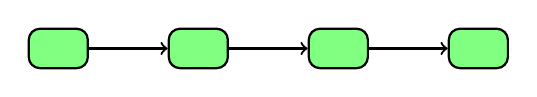
\begin{tikzpicture}
\tikzset{
  label/.style={text centered, text=orange,font=\footnotesize,minimum width=1cm} ,
  transform/.style={rectangle,rounded corners,draw=black,fill=green!50,text=white,thick, text centered, font=\tiny, minimum width=0.75cm,minimum height=0.5cm},
  item/.style={rectangle,draw=black,fill=orange!70,text=white,thick, text centered, font=\tiny, minimum width=0.75cm},
  result/.style={rectangle,draw=black,fill=blue!70,text=white,thick, text centered, font=\tiny, minimum width=0.75cm},
  arrow/.style={->,thick,draw=black,font=\tiny},
}  
\node[transform] (stage1) {};
\node[transform,right=1cm of stage1] (stage2) {};
\node[transform,right=1cm of stage2] (stage3) {};
\node[transform,right=1cm of stage3] (stage4) {};
%
\path[arrow] (stage1) -- (stage2);
\path[arrow] (stage2) -- (stage3);
\path[arrow] (stage3) -- (stage4);
\end{tikzpicture}
\end{center}
\end{frame}

\begin{frame}[t]{Standalone pipeline}
\begin{itemize}
  \item A \textmark{standalone} \textgood{pipeline} is a top-level pipeline.
    \begin{itemize}
      \item Invoking the pipeline translates into its execution.
    \end{itemize}

  \vfill\pause
  \item Given:
    \begin{itemize}
      \item A \textgood{generator} $g : \varnothing \mapsto T_1 \cup \varnothing$
      \item A sequence of \textgood{transformers} $t_i : T_i \mapsto T_{i+1}$
    \end{itemize}

  \vfill
  \item For every \textmark{non-empty} value generated by $g$, it evaluates:
    \begin{itemize}
      \item $t_n(t_{n-1}(\ldots t_1(g())))$
    \end{itemize}
\end{itemize}
\end{frame}

\begin{frame}[t,fragile]{Generators}
\begin{itemize}
  \item A generator $g$ is any callable C++ entity that:
    \begin{itemize}
      \item Takes no argument.
      \item Returns a value of type $T$ that may hold (or not) a value.
      \item Null value signals end of stream.
    \end{itemize}

  \vfill\pause
  \item The return value must be any type that:
    \begin{itemize}
      \item Is copy-constructible or move-constructible.
\begin{lstlisting}
T x = g();
\end{lstlisting}
      \pause
      \item Is contextually convertible to \cppkey{bool}
\begin{lstlisting}
if (x) { /*...*/ }
if (!x) { /*...*/ }
\end{lstlisting}
      \pause
      \item Can be derreferenced
\begin{lstlisting}
auto val = *x;
\end{lstlisting}
    \end{itemize}
  \vfill\pause
  \item The standard library offers an excellent candidate \cppid{std::experimental::optional<T>}.
\end{itemize}
\end{frame}

\begin{frame}[t,fragile]{Simple pipeline}
\begin{block}{x -> x*x -> 1/x -> print}
\begin{lstlisting}
template <typename Execution>
void run_pipe(const Execution & ex, int n)
{
  grppi::pipeline(ex,
    [i=0,max=n] () mutable -> optional<int> {
      if (i<max) return i++;
      else return {};
    },
    [](int x) -> double { return x*x; },
    [](double x) { return 1/x; },
    [](double x) { cout << x << "\n"; }
  );
}
\end{lstlisting}
\end{block}
\end{frame}

\begin{frame}[t,fragile]{Nested pipelines}
\begin{itemize}
  \item Pipelines may be nested.
  \vfill
  \item An inner pipeline:
    \begin{itemize}
      \item Does not take an execution policy.
      \item All stages are transformers (no generator).
      \item The last stage must also produce values.
    \end{itemize}
  \vfill
  \item The inner pipeline uses the same execution policy than the outer
        pipeline.
\end{itemize}
\end{frame}

\begin{frame}[t,fragile]{Nested pipelines}
\begin{block}{x -> x*x -> 1/x -> print}
\begin{lstlisting}
template <typename Execution>
void run_pipe(const Execution & ex, int n)
{
  grppi::pipeline(ex,
    [i=0,max=n] () mutable -> optional<int> {
      if (i<max) return i++;
      else return {};
    },
    grppi::pipeline(
      [](int x) -> double { return x*x; },
      [](double x) { return 1/x; }),
    [](double x) { cout << x << "\n"; }
  );
}
\end{lstlisting}
\end{block}
\end{frame}

\begin{frame}[t,fragile]{Piecewise pipelines}
\begin{itemize}
  \item A pipeline can be piecewise created.
\end{itemize}
\begin{block}{x -> x*x -> 1/x -> print}
\begin{lstlisting}
template <typename Execution>
void run_pipe(const Execution & ex, int n)
{
  auto generator = [i=0,max=n] () mutable -> optional<int> {
    if (i<max) return i++; else return {};
  };
  auto inner = grppi::pipeline(
      [](int x) -> double { return x*x; },
      [](double x) { return 1/x; });
  auto printer = [](double x) { cout << x << "\n"; };

  grppi::pipeline(ex, generator, inner, printer);
}
\end{lstlisting}
\end{block}
\end{frame}

%\begin{frame}[t]{Farm pattern}
\begin{itemize}
  \item A \textgood{farm} is a streaming pattern applicable to a stage in a \textmark{pipeline},
        providing multiple tasks to process data items from a data stream.
    \begin{itemize}
      \item A \textmark{farm} has an associated \textgood{cardinality} which is the number of parallel
             tasks used to serve the stage.
      \item Each task in a \textmark{farm} runs a \textgood{transformer} for each data item it receives.
    \end{itemize}
\end{itemize}
\end{frame}

\begin{frame}[t,fragile]{Farms in pipelines}
\begin{block}{Square values}
\begin{lstlisting}
template <typename Execution>
void run_pipe(const Execution & ex, int n)
{
  grppi::pipeline(ex,
    [i=0,max=n] () mutable -> optional<int> {
      if (i<max) return i++;
      else return {};
    },
    grppi::farm(4
      [](int x) -> double { return x*x; }),
    [](double x) { cout << x << "\n"; }
  );
}
\end{lstlisting}
\end{block}
\end{frame}

\begin{frame}[t,fragile]{Piecewise farms}
\begin{block}{Square values}
\begin{lstlisting}
template <typename Execution>
void run_pipe(const Execution & ex, int n)
{
  auto inner = grppi::farm(4 [](int x) -> double { return x*x; });

  grppi::pipeline(ex,
    [i=0,max=n] () mutable -> optional<int> {
      if (i<max) return i++;
      else return {};
    },
    inner,
    [](double x) { cout << x << "\n"; }
  );
}
\end{lstlisting}
\end{block}
\end{frame}

%\begin{frame}[t]{Ordering}
\begin{itemize}
  \item Signals if pipeline items must be consumed in the same order they were produced.
    \begin{itemize}
      \item Do they need to be \emph{time-stamped}?
    \end{itemize}

  \vfill
  \item Default is \textmark{ordered}.

  \vfill
  \item \textenum{API}
    \begin{itemize}
      \item \cppid{ex.enable\_ordering()}
      \item \cppid{ex.disable\_ordering()}
      \item \cppkey{bool } \cppid{o = ex.is\_ordered()}
    \end{itemize}
\end{itemize}
\end{frame}

\begin{frame}[t]{Queueing properties}
\begin{itemize}
  \item Some policies (\textgood{native} and \textgood{omp}) use queues to
        communicate pipeline stages.

  \vfill
  \item \textenum{Properties}:
    \begin{itemize}
      \item \textmark{Queue size}: Buffer size of the queue.
      \item \textmark{Mode}: \emph{blocking} versus \emph{lock-free}.
    \end{itemize}

  \vfill
  \item \textenum{API}
    \begin{itemize}
      \item \cppid{ex.set\_queue\_attributes(100, mode::blocking)}
    \end{itemize}
\end{itemize}
\end{frame}

%\subsection{Filtering stages}

\begin{frame}[t]{Filter pattern}
\begin{itemize}
  \item A \textgood{filter} pattern discards (or keeps) the data items from a 
        data stream based on the outcome of a predicate.
  \item This pattern can be used only as a stage of a \textmark{pipeline}.
  \vfill\pause
  \item \textenum{Alternatives}:
    \begin{itemize}
      \item \textmark{Keep}: Only data items satisfying the predicate are sent 
            to the next stage.
      \item \textmark{Discard}: Only data items \textbf{\alert{not satisfying}} 
            the predicate are sent to the next stage.
    \end{itemize}
\end{itemize}
\end{frame}

\begin{frame}[t,fragile]{Filtering in}
\begin{block}{Print primes}
\begin{lstlisting}
bool is_prime(int n);

template <typename Execution>
void print_primes(const Execution & ex, int n)
{
  grppi::pipeline(exec,
    [i=0,max=n]() mutable -> optional<int> {
      if (i<=n) return i++;
      else return {};
    },
    grppi::keep(is_prime),
    [](int x) { cout << x << "\n"; }
  );
}
\end{lstlisting}
\end{block}
\end{frame}

\begin{frame}[t,fragile]{Filtering out}
\begin{block}{Discard words}
\begin{lstlisting}
template <typename Execution>
void print_primes(const Execution & ex, std::istream & is)
{
  grppi::pipeline(exec,
    [&file]() -> optional<string> {
      string word;
      file >> word;
      if (!file) { return {}; }
      else { return word; }
    },
    grppi::discard([](std::string w) { return w.length() < 4; },
    [](std::string w) { cout << x << "\n"; }
  );
}
\end{lstlisting}
\end{block}
\end{frame}

%\subsection{Reductions in pipelines}

\begin{frame}[t]{Stream reduction pattern}
\begin{itemize}
  \item A \textgood{stream reduction} pattern performs a reduction over the items of a
        subset of a data stream.
  \vfill\pause
  \item \textenum{Key elements}
    \begin{itemize}
      \item \textmark{window-size}: Number of elements in a reduction window.
      \item \textmark{offset}: Distance between two consecutive window starts.
      \item \textmark{identity}: Value used as identity in reductions.
      \item \textmark{combiner}: Combination operation used for reductions.
    \end{itemize}
\end{itemize}
\end{frame}

\begin{frame}[t,fragile]{Windowed reductions}
\begin{block}{Chunked sum}
\begin{lstlisting}
template <typename Execution>
void print_primes(const Execution & ex, int n)
{
  grppi::pipeline(exec,
    [i=0,max=n]() mutable -> optional<double> {
      if (i<=n) return i++;
      else return {};
    },
    grppi::reduce(100, 50, 0.0,
      [](double x, double y) { return x+y; }),
    [](int x) { cout << x << "\n"; }
  );
}
\end{lstlisting}
\end{block}
\end{frame}

%\subsection{Iterations in pipelines}

\begin{frame}[t]{Stream iteration pattern}
\begin{itemize}
  \item A \textgood{stream iteration} pattern allows loops in data stream processing.
    \begin{itemize}
      \item An operation is applied to a data item until a predicate is satisfied.
      \item When the predicate is met, the result is sent to the output stream.
    \end{itemize}
  \vfill\pause
  \item \textenum{Key elements}:
    \begin{itemize}
      \item A \textmark{transformer} that is applied to a data item on each iteration.
      \item A \textmark{predicate} to determine when the iteration has finished.
    \end{itemize}
\end{itemize}
\end{frame}

\begin{frame}[t,fragile]{Iterating}
\begin{block}{Print values $2^n*x$}
\begin{lstlisting}
template <typename Execution>
void print_values(const Execution & ex, int n)
{
  auto generator = [i=1,max=n+1]() mutable -> optional<int> {
    if (i<max) return i++;
    else return {};
  };

  grppi::pipeline(ex,
    generator,
    grppi::repeat_until(
      [](int x) { return 2*x; },
      [](int x) { return x>1024; }
    ),
    [](int x) { cout << x << endl; }
  );
}
\end{lstlisting}
\end{block}
\end{frame}


\section{Writing your own execution}

\begin{frame}[t]{Addine a new policy}
\begin{itemize}
\item Adding a new execution policy is done by writing a new class.
  \begin{itemize}
    \item No inheritance needed.
      \begin{itemize}
        \item \emph{``Inheritance is the base class of all evils''} (Sean Parent).
      \end{itemize}
    \item No dependency from the library.
    \item Additionally configure some meta-functions (until we have concepts).
  \end{itemize}
\end{itemize}
\end{frame}

\begin{frame}[t,fragile]{My custom execution}
\begin{block}{my\_execution}
\begin{lstlisting}
class my_execution {
  my_execution() noexcept;

  void set_concurrency_degree(int n) const noexcept;
  void concurrency_degree() const noexcept;

  void enable_ordering() noexcept;
  void disable_ordering() noexcept;
  bool is_ordered() const noexcept;

  //...
};

template <>
constexpr bool is_supported<my_execution>() { return true; }
\end{lstlisting}
\end{block}
\end{frame}

\begin{frame}[t,fragile]{Adding a pattern}
\begin{block}{my\_execution::map}
\begin{lstlisting}
class my_execution {

  // ...

  template <typename ... InputIterators, typename OutputIterator, 
            typename Transformer>
  constexpr void map(std::tuple<InputIterators...> firsts,
      OutputIterator first_out, std::size_t sequence_size, 
      Transformer && transform_op) const;

  //...
};

template <>
constexpr bool supports_map<my_execution>() { return true; }
\end{lstlisting}
\end{block}
\end{frame}

\begin{frame}[t,fragile]{Some helpers in the library}
\begin{block}{Applying a function to a tuple of iterators}
\begin{lstlisting}
template <typename F, typename ... Iterators, template <typename ...> class T>
decltype(auto) apply_deref_increment(
    F && f, 
    T<Iterators...> & iterators)
\end{lstlisting}
\end{block}
\vfill
\begin{itemize}
  \item Takes a function \cppid{f} and a tuple of iterators (e.g. result of \cppid{make\_tuple(it1, it2, it3)}.
  \item Returns \cppid{f(*it1++, *it2++, *it3++)}.
  \item Very convenient for implementing data patterns.
  \item More like this in \cppid{include/common/iterator.h}.
\end{itemize}
\end{frame}


\begin{frame}[t,fragile]{Implementing map}
\begin{block}{map}
\begin{lstlisting}
template <typename ... InputIterators, typename OutputIterator, 
          typename Transformer>
void my_execution_native::map(std::tuple<InputIterators...> firsts,
    OutputIterator first_out, std::size_t sequence_size, 
    Transformer transform_op) const
{
  using namespace std;
  auto process_chunk = [&transform_op](auto fins, std::size_t size, auto fout)
  {
    const auto l = next(get<0>(fins), size);
    while (get<0>(fins)!=l) {
      *fout++ = apply_deref_increment(
          std::forward<Transformer>(transform_op), fins);
    }
  };
  //...
\end{lstlisting}
\end{block}
\end{frame}

\begin{frame}[t,fragile]{Implementing map}
\begin{block}{map}
\begin{lstlisting}
  //...
  const int chunk_size = sequence_size / concurrency_degree_;
  {
    some_worker_pool workers;
    for (int i=0; i!=concurrency_degree_-1; ++i) {
      const auto delta = chunk_size * i;
      const auto chunk_firsts = iterators_next(firsts,delta);
      const auto chunk_first_out = next(first_out, delta);
      workers.launch(process_chunk, chunk_firsts, chunk_size, chunk_first_out);
    }

    const auto delta = chunk_size * (concurrency_degree_ - 1);
    const auto chunk_firsts = iterators_next(firsts,delta);
    const auto chunk_first_out = next(first_out, delta);
    process_chunk(chunk_firsts, sequence_size - delta, chunk_first_out);
  } // Implicit pool synch
}

\end{lstlisting}
\end{block}
\end{frame}


\section{Conclusions}

\begin{frame}[t]{Summary}
\begin{itemize}
  \item An unified programming model for sequential and parallel modes.
  \item Multiple back-ends available.
  \item Current pattern set:
    \begin{itemize}
      \item \textenum{Data}: \textmark{map}, \textmark{reduce}, \textmark{map/reduce}, \textmark{stencil}.
      \item \textenum{Task}: \textmark{divide/conquer}.
      \item \textenum{Streaming}: \textmark{pipeline} with nesting of \textmark{farm}, \textmark{filter},
            \textmark{reduction}, \textmark{iteration}.
    \end{itemize}
\end{itemize}
\end{frame}

\begin{frame}{GrPPI}
\begin{Large}
\textgood{\url{https://github.com/arcosuc3m/grppi}}
\end{Large}
\end{frame}



\begin{frame}
\titlepage
\end{frame}

\section{Evaluation}

\begin{frame}[t]{Evaluation platform}
\begin{itemize}
  \item \textenum{Plataforma}:
    \begin{itemize}
      \item 2 $\times$ Intel Xeon Ivy Bridge E5-2695 v2.
      \item \textmark{Number of cores}: 24.
      \item \textmark{Clock frequency}: 2.40 GHz.
      \item \textmark{L3 cache size}: 30 MB.
      \item \textmark{Main memory}: 128 GB DDR3.
      \item OS: Ubuntu Linux 14.04 LTS, kernel 3.13.
    \end{itemize}

  \vfill
  \item \textenum{Compiler}: GCC 5.0.
    \begin{itemize}
      \item \textgood{OpenMP}: GCC.
      \item \textgood{ISO C++ Threads}: GCC.
      \item \textgood{Intel TBB}: \textmark{\url{www.threadingbuildingblocks.org}}
    \end{itemize}
\end{itemize}
\end{frame}

\begin{frame}[t]{Example}
\begin{itemize}
  \item Video frame processing for border detection with two filters.
    \begin{itemize}
      \item Gaussian blur.
      \item Sobel.
    \end{itemize}
  \vfill\pause
  \item Using \textgood{pipeline} pattern:
    \begin{itemize}
      \item S1: Frame reading.
      \item S2: Gaussian blur (may apply \textgood{farm}).
      \item S3: Sobel filter (may apply \textgood{farm}).
      \item S4: Frame writing.
    \end{itemize}
  \vfill\pause
  \item \textenum{Approaches}:
    \begin{itemize}
      \item Manual.
      \item \textmark{GrPPI}.
    \end{itemize}
\end{itemize}
\end{frame}

\begin{frame}{Esfuerzo de paralelización}
\begin{tabular}{|c|r|r|r|r|}
\hline
Pipeline & \multicolumn{4}{c|}{\centering\let\newline\\ \% LOC increase} \\\cline{2-5}
Composition & \textbf{C++ Threads}  & \textbf{OpenMP} & \textbf{Intel TBB}  & \textbf{GrPPI} \\\hline\hline
\texttt{(\,p\,$|$\,p\,$|$\,p\,$|$\,p\,)} & $+$8.8\,\%   & $+$13.0\,\%  & $+$25.9\,\% & $+$1.8\,\% \\
\texttt{(\,p\,$|$\,f\,$|$\,p\,$|$\,p\,)} & $+$59.4\,\%  & $+$62.6\,\%  & $+$25.9\,\% & $+$3.1\,\% \\
\texttt{(\,p\,$|$\,p\,$|$\,f\,$|$\,p\,)} & $+$60.0\,\%  & $+$63.9\,\%  & $+$25.9\,\% & $+$3.1\,\% \\
\texttt{(\,p\,$|$\,f\,$|$\,f\,$|$\,p\,)} & $+$106.9\,\% & $+$109.4\,\% & $+$25.9\,\% & $+$4.4\,\% \\\hline
\end{tabular}
\end{frame}

\begin{frame}{Performance: frames per second}
\includegraphics[height=.85\textheight]{fps.pdf}
\end{frame}

%\begin{frame}{Observaciones}
%\begin{itemize}
%  \item Impacto del patrón \textgood{farm}:
%    \begin{itemize}
%      \item El uso de \textgood{farm} en ambas etapas causa una mejora sustancial del rendimiento.
%        \begin{itemize}
%          \item Equilibrio.
%        \end{itemize}
%      \item El uso de \textgood{farm} en una única etapa del pipeline no tiene impacto significativo.
%        \begin{itemize}
%          \item Desequilibrio.
%        \end{itemize}
%    \end{itemize}
%
%  \vfill\pause
%  \item Impacto de GrPPI en el rendimento.
%    \begin{itemize}
%      \item Sobrecoste por debajo del 2\%.
%    \end{itemize}
%
%  \vfill\pause
%  \item Impacto en el esfuerzo.
%    \begin{itemize}
%      \item Reducción significativa con respecto a los otros enfoques de programación.
%    \end{itemize}
%\end{itemize}
%\end{frame}
%
%\begin{frame}[t]{Conclusiones}
%\begin{itemize}
%  \item GrPPI permite cambiar de modelo de programación subyacente con mínimo esfuerzo
%        gracias al uso de C++ moderno.
%  \vfill\pause
%  \item Diseño compacto para ocultar la complejidad de alternativas de implementación.
%  \vfill\pause
%  \item Soporte de múltiples patrones:
%    \begin{itemize}
%      \item \textenum{Datos/}: \textmark{map}, \textmark{reduce}, \textmark{map/reduce}, \textmark{stencil}.
%      \item \textenum{Tareas}: \textmark{divide/conquer}.
%      \item \textenum{streaming} \textmark{pipeline} con etapas \textmark{farm}, \textmark{filter}, \textmark{reduce},
%                                 \textmark{iteration}.
%    \end{itemize}
%  \vfill\pause
%  \item Mínimo sobrecoste de:
%    \begin{itemize}
%      \item Modificaciones del código fuente.
%      \item Rendimiento.
%    \end{itemize}
%\end{itemize}
%\end{frame}
%
%\begin{frame}[t]{Trabajo futuro}
%\begin{itemize}
%  \item Mejorar y ampliar políticas de ejecución (Thrust, FastFlow, \ldots).
%  \item Incorporar nuevos patrones.
%  \item Extender y simplificar la interfaz para patrones de datos.
%  \item Dar soporte a combinación de políticas de ejecución.
%  \item Mejorar el soporte NUMA.
%  \item Ampliar aplicaciones ejemplo y benchmarks.
%  \vfill
%  \item \textgood{\url{https:/www.github.com/arcosuc3m/grppi}}.
%\end{itemize}
%\end{frame}


\end{document}
\grid
